\documentclass[conference]{IEEEtran}

\usepackage{amsmath}
\usepackage{array}
\usepackage{booktabs}
\usepackage{cite}
\usepackage{graphicx}
\usepackage{url}
\usepackage{xcolor}
\newcolumntype{L}[1]{>{\raggedright\arraybackslash}p{#1}}

\title{Deep Learning-Based Black-Box Modelling for Instrument Tone Transformation: A Literature Review}

\author{
\IEEEauthorblockN{YangJunyan 2330034063}
}

\begin{document}
\raggedbottom

\maketitle

\begin{abstract}
Deep learning-based black-box audio modelling has become a practical approach for reproducing nonlinear instrument tones without deriving a physical or circuit-level description of the target device. This literature review examines the technical basis for NeuralToneTransform, whose design goal is to transform ordinary instrument inputs into high-fidelity target tones while preserving expressive detail and evaluating real-time feasibility. The review focuses on guitar amplifiers, distortion pedals, cabinets, and nonlinear audio effects because this area offers the most mature evidence base for the broader tone-transformation problem. It covers recurrent networks, long short-term memory models, WaveNet-style and temporal convolutional networks, the Neural Amp Modeler open-source ecosystem, paired-data collection, sample-level alignment, loss functions, evaluation practice, timbre transfer, and differentiable digital signal processing. The current project has reproduced a Neural Amp Modeler baseline, but it has not yet implemented an independent TCN, WaveNet, or LSTM model, a self-collected paired dataset, or a final inference and evaluation system. The literature suggests that the central gap is methodological: a credible system must combine accurate alignment, perceptually meaningful objectives, controlled evaluation, and latency-aware architecture design.
\end{abstract}

\begin{IEEEkeywords}
black-box modelling, audio effects, guitar amplifier modelling, neural networks, WaveNet, temporal convolutional networks, LSTM, Neural Amp Modeler, tone transformation
\end{IEEEkeywords}

\section{Introduction}

Musical tone is shaped by the instrument, pickup, amplifier, cabinet, microphone, room, and effects chain. Ordinary or low-cost instruments cannot always produce the target tones associated with premium orchestral instruments, classic synthesizers, high-end guitar amplifiers, or carefully recorded studio chains. A performance-oriented system must therefore do more than change spectral colour. It must preserve dynamics, articulation, transient behaviour, note decay, and other playing nuances. NeuralToneTransform is motivated by this problem. The proposed project asks whether deep learning-based black-box modelling can support instrument tone transformation while treating real-time operation as an evaluation target.

Traditional physical modelling and circuit modelling remain important in digital audio effects. They provide interpretability, explicit control, and predictable behaviour when the target device is well understood. However, detailed models of vacuum-tube amplifiers, distortion circuits, loudspeaker cabinets, microphones, and production chains are difficult to construct. These systems may include nonlinearities, memory effects, component tolerances, and undocumented design choices. Black-box modelling offers a complementary route. Instead of deriving internal equations, it learns the input-output mapping from paired dry and wet audio. This makes it attractive when the external behaviour of a device is easier to observe than its internal mechanism.

This review focuses mainly on guitar amplifier, distortion pedal, cabinet, and nonlinear audio effect modelling. These tasks do not cover the entire ambition of instrument tone transformation, but they provide a mature and technically relevant subset of the problem. The literature contains direct comparisons between recurrent neural networks (RNNs), long short-term memory (LSTM) networks, WaveNet-style convolutional models, temporal convolutional networks (TCNs), and practical open-source systems. These methods align with the intended next stage of NeuralToneTransform, where the current Neural Amp Modeler (NAM) baseline should be followed by an independently explained TCN, WaveNet, or LSTM model and a transparent evaluation pipeline. The review therefore treats NAM as a strong engineering baseline and software ecosystem, not as the complete research contribution.

The reference order follows the technical progression used in this review: raw waveform modelling and TCNs \cite{oord2016wavenet,bai2018tcn}, recurrent amplifier models \cite{schmitz2018lstm,wright2019rnn,wright2020guitar}, neural black-box audio effects \cite{ramirez2018nonlinear,ramirez2020blackbox,vanhatalo2022review}, differentiable digital signal processing \cite{engel2020ddsp}, and the NAM software ecosystem \cite{atkinson_nam}.

The review uses an algorithmic-methods perspective rather than a product demonstration perspective. Each model family is assessed by the type of temporal dependency it can represent, the data assumptions it makes, and the evaluation risks it creates. This framing is important for a Final Year Project because a working baseline alone does not establish scientific contribution. The contribution must come from a justified modelling choice, a reproducible data pipeline, and a fair comparison with measured limitations.

The current project status must be stated carefully. At this stage, the environment setup and official NAM baseline reproduction have been completed. The project has not yet implemented a self-developed TCN, WaveNet, or LSTM model, a self-collected paired dry/wet dataset, sample-level alignment, ESR/DC loss training, real-time inference, or final evaluation. The purpose of this paper is therefore to establish the theoretical and technical foundation for later work rather than to report completed modelling results.

\section{Audio Black-Box Modelling and Nonlinear Audio Effects}

Black-box audio modelling learns a function from an input signal $x[n]$ to a target signal $y[n]$ without explicitly modelling the circuit, acoustic structure, or algorithm that produced $y[n]$. In supervised neural audio effect modelling, the training data typically consist of paired dry and wet recordings. The dry signal is passed through the target device, plugin, or signal chain, and the model is trained to reproduce the wet output. Martinez Ramirez and Reiss framed this as an end-to-end learning problem for nonlinear audio effects \cite{ramirez2018nonlinear}. Martinez Ramirez, Benetos, and Reiss later generalised the discussion to black-box modelling and compared neural architectures across multiple effect types \cite{ramirez2020blackbox}.

Nonlinear audio systems are challenging because their output is not a simple scaled or filtered version of the input. Tube amplifiers, overdrive pedals, fuzz circuits, compressors, and loudspeaker cabinets can produce harmonic distortion, intermodulation, dynamic saturation, hysteresis-like memory, frequency-dependent gain, and transient-dependent responses. Guitar systems are especially demanding because playing techniques such as palm muting, vibrato, bends, pick attack, chord voicing, and volume-knob changes can alter both the amplitude envelope and spectral content. Vanhatalo \emph{et al.} emphasise that neural amplifier emulation must be understood in relation to black-box, grey-box, and white-box modelling approaches, each of which makes different assumptions about access to system structure and data \cite{vanhatalo2022review}.

Deep learning is suitable for this class of problem because neural networks can approximate complex nonlinear time-domain mappings. In raw waveform modelling, the model receives samples or short sequences and predicts corresponding output samples. This avoids manually selecting a small set of spectral features, which may discard relevant phase or transient information. However, the same flexibility creates practical risks. A model can learn dataset artefacts, timing errors, noise, or device-specific biases if the data are poorly aligned or insufficiently diverse. Consequently, black-box modelling should be treated as a complete pipeline involving data design, alignment, model architecture, training loss, validation, latency measurement, and listening evaluation.

This pipeline view also clarifies the boundary between literature review and implementation. The reviewed work supports the feasibility of neural emulation, but it does not remove the need for project-specific validation. A student system must still show that its dataset excites the target behaviour, that its delay compensation is correct, and that its metrics reflect the intended listening task.

Fig.~\ref{fig:pipeline} summarises the pipeline implied by the reviewed literature and the intended direction of this project. The dry instrument signal is recorded or generated, passed through a target tone device or re-amping path, aligned with the resulting wet signal, segmented into training examples, and used to train a model. The trained model must then be assessed through objective and subjective evaluation rather than assumed to be perceptually accurate.

\begin{figure*}[t]
  \centering
  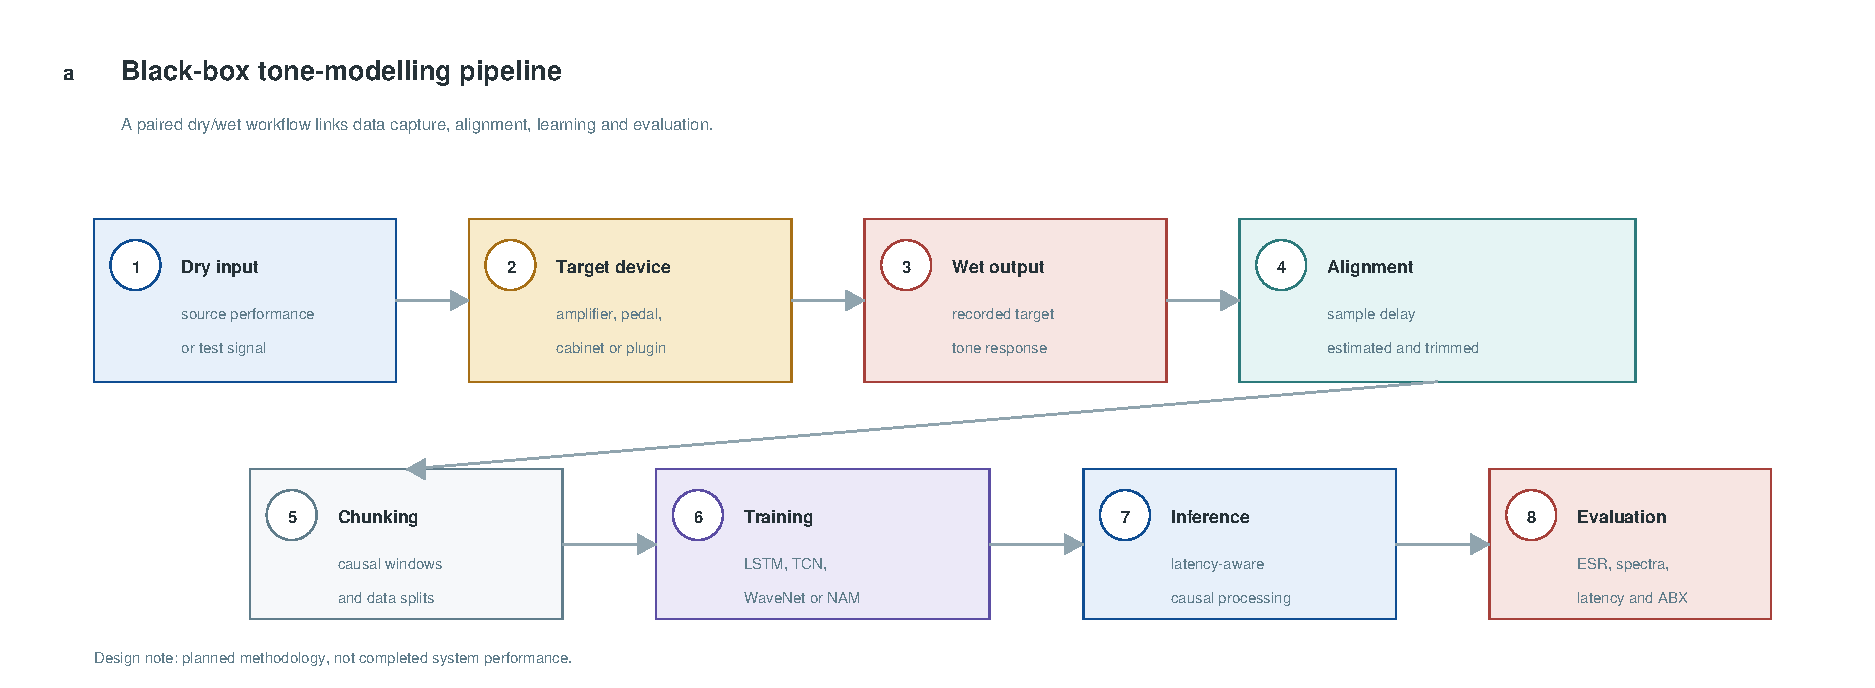
\includegraphics[width=0.95\textwidth]{figures/pipeline.pdf}
  \caption{Supervised black-box tone-modelling workflow. The panel presents the planned evidence chain from paired recording to evaluation; it does not report completed system results.}
  \label{fig:pipeline}
\end{figure*}

\section{Recurrent Neural Networks and LSTM for Real-Time Audio Modelling}

RNNs are natural candidates for audio effect modelling because time-domain audio systems often depend on previous samples. Unlike a memoryless nonlinear function, an amplifier or dynamic effect may respond differently to the same instantaneous amplitude depending on recent signal history. LSTM and gated recurrent unit (GRU) architectures address vanishing-gradient limitations in basic RNNs and maintain internal state over time. This memory makes them relevant for nonlinear audio devices with short- and medium-term dependencies.

Schmitz and Embrechts used an LSTM network for real-time emulation of a parametric guitar tube amplifier, treating the amplifier as a nonlinear system whose behaviour can be learned from examples \cite{schmitz2018lstm}. Wright, Damsk{\"a}gg, and V{\"a}lim{\"a}ki later presented real-time black-box modelling with recurrent neural networks and demonstrated their relevance to tube amplifier and distortion pedal modelling \cite{wright2019rnn}. Wright \emph{et al.} extended this line of work by comparing recurrent and WaveNet-style approaches for guitar amplifier emulation, including discussion of real-time implementation considerations \cite{wright2020guitar}.

The main advantage of LSTM-based models is efficient sequential processing. A compact recurrent model can process one sample at a time while carrying hidden state forward. This is useful for low-latency audio because a causal implementation does not require a large look-ahead buffer. The recurrent state also provides a direct mechanism for memory effects, which are important in amplifier and effect modelling. For a student project, an LSTM can serve as a clear baseline because it is conceptually linked to system memory and has already been applied to similar audio tasks.

The weakness of recurrent models is that very long effective receptive fields can be difficult to learn and optimise. Although LSTM gates help retain information, they do not guarantee that the model will use long histories effectively. Bai, Kolter, and Koltun argued more broadly that convolutional sequence models can outperform canonical recurrent networks on several sequence-modelling tasks while demonstrating longer effective memory \cite{bai2018tcn}. In audio black-box modelling, this suggests that an LSTM baseline should be compared with dilated convolutional models rather than treated as the final architecture by default.

For NeuralToneTransform, this comparison should be framed as a design test rather than a competition for a universal best model. An LSTM may be preferable if compactness and implementation simplicity dominate. A TCN may be preferable if longer context and training parallelism dominate. The project should therefore report the conditions under which each model is evaluated, including block size, sampling rate, parameter count, and latency measurement method.

\section{WaveNet and Temporal Convolutional Networks for Raw Waveform Modelling}

WaveNet introduced a powerful raw waveform modelling framework based on causal and dilated convolutions \cite{oord2016wavenet}. A causal convolution ensures that the output at time $n$ depends only on current and past inputs. This is essential for real-time audio systems that cannot depend on future samples. Dilation increases the spacing between filter taps, allowing a network to cover a large temporal context without a very long dense filter. When dilation rates grow exponentially, such as 1, 2, 4, and 8, the receptive field expands rapidly.

TCNs generalise this idea for sequence modelling by using causal convolutional layers, dilation, residual connections, and stable training procedures. Bai \emph{et al.} showed that convolutional sequence models should be considered strong alternatives to recurrent models, particularly where long history is useful \cite{bai2018tcn}. For audio tone transformation, this is technically important because amplifier and cabinet responses may involve both short nonlinear distortion and longer impulse-response-like behaviour. A causal dilated network can model sample-level nonlinearities while also seeing enough past context to reproduce resonances and transients.

WaveNet-style models have been directly studied for guitar amplifier emulation. Wright \emph{et al.} compared WaveNet-style feedforward models with recurrent models and analysed receptive field, activation functions, and real-time implementation trade-offs \cite{wright2020guitar}. Their work is especially relevant to NeuralToneTransform because the planned independent model direction includes causal convolution, dilation, gated activation, residual connection, and skip connection. These components provide a coherent path from the literature to an implementable student baseline.

The main implementation risk is that receptive field and latency are linked but not identical. A model can have a large past context and still operate causally, yet its compute cost may exceed a practical audio buffer budget. The literature therefore supports evaluating convolutional models at both signal level and system level. Signal-level tests measure waveform and spectral similarity, while system-level tests measure block processing time and stability under continuous input.

Fig.~\ref{fig:dilation} illustrates the central idea. Each layer uses a causal connection pattern, but the dilation factor changes the spacing between accessed samples. With increasing dilation, the model can use a wider history while keeping the number of parameters and operations manageable. In practice, the exact receptive field should be chosen according to the target system and measured latency constraints.

\begin{figure*}[t]
  \centering
  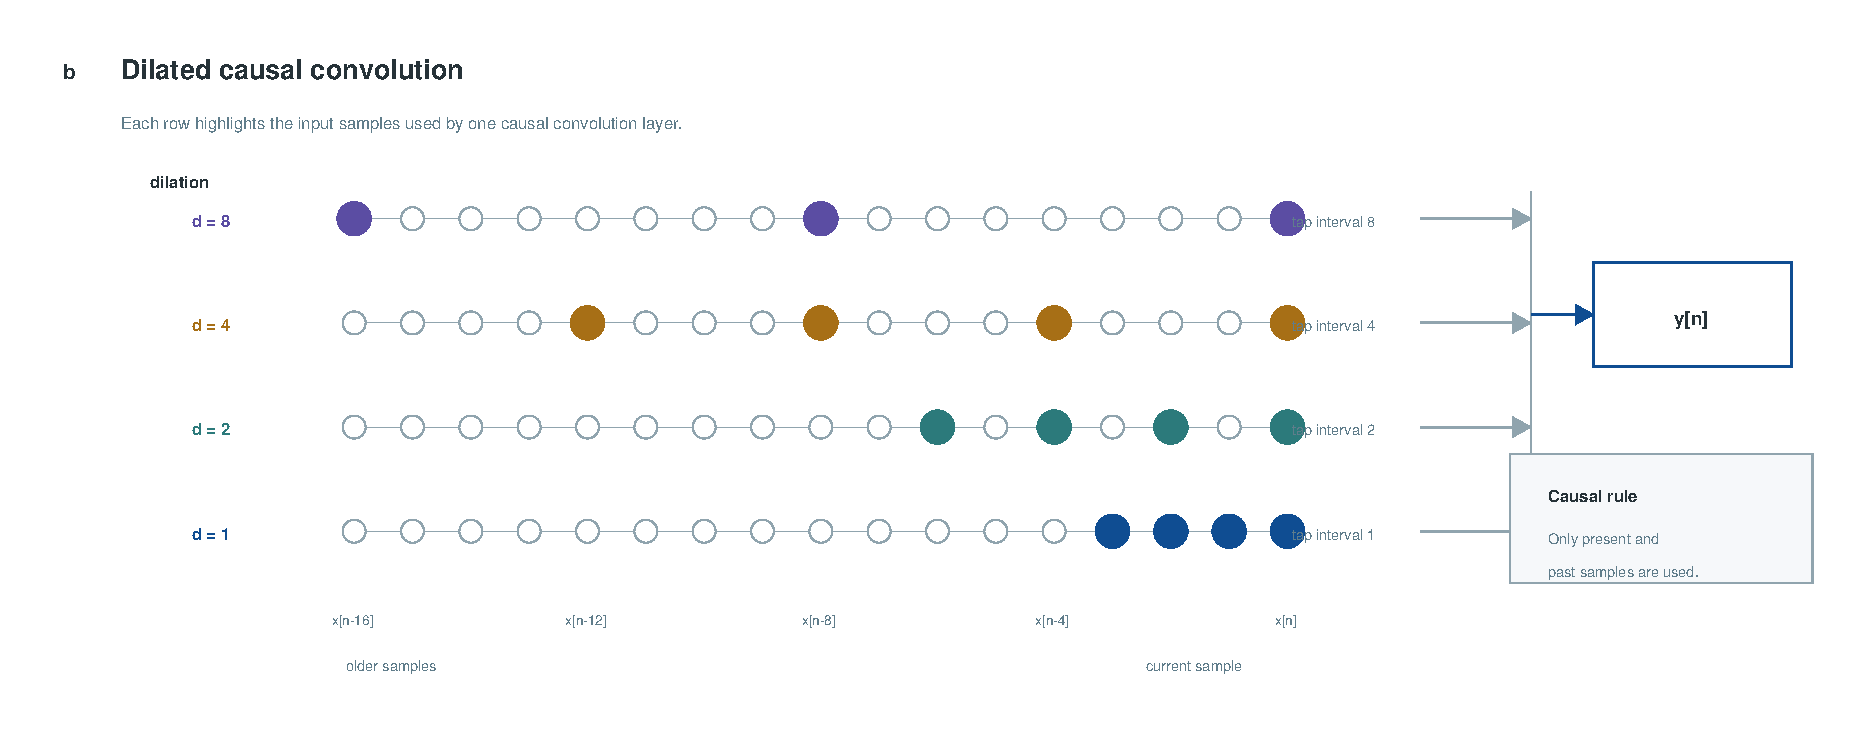
\includegraphics[width=0.90\textwidth]{figures/dilated_causal_convolution.pdf}
  \caption{Dilated causal convolution with dilation rates 1, 2, 4, and 8. The visual claim is receptive-field expansion under causal operation, which is necessary for real-time feasibility.}
  \label{fig:dilation}
\end{figure*}

\section{Neural Amp Modeler and Open-Source Guitar Tone Modelling Ecosystems}

Neural Amp Modeler is an open-source neural network emulator for guitar amplifiers and related devices. The official repository describes NAM as software for training models and exporting them to \texttt{.nam} files. The associated website presents NAM as an open-source deep learning project for modelling guitar amplifiers and pedals \cite{atkinson_nam}. NAM is highly relevant to NeuralToneTransform because the current project has already reproduced the official NAM baseline. This makes NAM a practical reference point for environment setup, dataset expectations, model packaging, and user-facing guitar tone modelling workflows.

However, a baseline reproduction is not the same as an independent research contribution. NAM should be treated as a strong engineering baseline and ecosystem rather than the only contribution of the Final Year Project. Its value is that it gives the project a working reference implementation and a realistic target domain. Its limitation in this academic context is that merely running an existing open-source tool does not explain the design choices, data alignment strategy, loss functions, architecture comparison, or evaluation methodology required for a complete project.

The future work of NeuralToneTransform should therefore use NAM as a benchmark against which simpler and independently implemented models can be compared. A self-developed LSTM or TCN model can expose architectural decisions more clearly than a full production ecosystem. NAM can remain useful for baseline reproduction and practical comparison, while the academic report should explain why the independent pipeline is necessary. This positioning avoids overclaiming and aligns the project with both engineering realism and educational assessment.

This distinction also protects the evaluation logic. If the self-developed model performs worse than NAM, the result can still be informative if the comparison identifies why. Possible causes include insufficient receptive field, inadequate alignment, weak dataset coverage, or an unsuitable loss function. The project should therefore use NAM as an anchor for analysis rather than as a shortcut around model explanation.

\section{Data Collection, Re-Amping, and Sample-Level Alignment}

Data quality is central to black-box audio modelling. In supervised learning, the model can only learn behaviours represented in the paired dry and wet dataset. For guitar and instrument tone transformation, a dataset should cover frequency range, dynamic range, transients, sustain, silence, noise, single notes, chords, palm mutes, bends, pickup positions, and representative playing styles. If the dry input does not excite a behaviour of the target system, the model is unlikely to reproduce that behaviour reliably. Martinez Ramirez \emph{et al.} highlight black-box audio effects as a supervised learning problem in which training examples must represent the target effect behaviour \cite{ramirez2020blackbox}.

Re-amping is a practical way to obtain paired data. A clean direct-input guitar or keyboard signal can be recorded first, then played back through a target amplifier, pedal, cabinet simulator, or plugin chain to produce the wet target. This approach allows the same dry performance to be processed through multiple target devices and settings. Wright \emph{et al.} use paired input-output data for modelling guitar amplifiers and effects, reinforcing the importance of controlled recording and train/test separation \cite{wright2020guitar}. Vanhatalo \emph{et al.} further show that data-driven amplifier emulation depends heavily on the relationship between target systems, network class, and measurement conditions \cite{vanhatalo2022review}.

Sample-level alignment is essential. Even a small delay between the dry input and wet target can cause the model to learn an incorrect mapping. In time-domain losses, a target signal shifted by a few samples may produce a large error even if it sounds nearly identical, while the model may be incorrectly penalised for predicting the right waveform at the wrong time. Cross-correlation is an appropriate method for estimating delay between paired signals because it finds the relative lag that maximises similarity. Once the lag is estimated, the signals can be trimmed or shifted before chunking.

Train, validation, and test splitting should be planned before training. The training set is used for parameter learning, the validation set for model selection and early stopping, and the test set for final evaluation. Splits should avoid leakage. For example, near-identical chunks from the same performance should not appear in both training and test sets if the goal is to evaluate generalisation. For this project, dataset design and alignment are not auxiliary engineering details. They are part of the core research methodology.

Practical dataset preparation should also record gain staging and normalisation choices. A nonlinear device may react differently to level changes, so arbitrary loudness normalisation can change the task being learned. Silence and low-level noise should not be removed automatically, because offset, hiss, and decay behaviour may be part of the target response. These details should be documented with the same care as model hyperparameters.

\section{Loss Functions and Evaluation Methods}

Simple mean squared error (MSE) is easy to optimise but is not always sufficient for perceptual audio quality. A small time-domain error does not guarantee preservation of attack, brightness, saturation texture, or perceived realism. Conversely, a perceptually acceptable signal may still produce a high sample-wise error if there is a small phase or alignment difference. Audio black-box modelling therefore often combines time-domain losses with additional checks.

Error-to-signal ratio (ESR) is commonly used in virtual analog and audio effect modelling because it normalises the prediction error by the target signal energy. A typical form is
\begin{equation}
\mathrm{ESR} = \frac{\sum_n (y[n] - \hat{y}[n])^2}{\sum_n y[n]^2 + \epsilon},
\end{equation}
where $y[n]$ is the target wet signal, $\hat{y}[n]$ is the model prediction, and $\epsilon$ prevents division by zero. DC loss can complement ESR by discouraging offset errors:
\begin{equation}
\mathcal{L}_{\mathrm{DC}} = \left(\frac{1}{N}\sum_n y[n] - \frac{1}{N}\sum_n \hat{y}[n]\right)^2.
\end{equation}
These losses are relevant to NeuralToneTransform because planned ESR/DC training should directly follow established audio effect modelling practice rather than use generic MSE alone \cite{wright2020guitar,ramirez2020blackbox}.

Frequency-domain and spectrogram-based comparisons can complement time-domain losses. They can reveal whether the model captures harmonic distortion, resonant peaks, high-frequency roll-off, and noise-like artefacts. However, frequency-domain metrics also have limitations because they may not fully capture phase, timing, transient sharpness, or playing feel. Vanhatalo \emph{et al.} emphasise that amplifier emulation evaluation must consider both technical and perceptual dimensions \cite{vanhatalo2022review}.

Subjective listening tests are therefore important. ABX tests are useful because listeners compare two known references, A and B, with an unknown X and decide whether X matches A or B. In this project, ABX or preference tests could compare target wet audio, NAM baseline output, and self-developed model output. The evaluation should include model accuracy, perceptual quality, computational cost, and latency. Importantly, the project should not claim ultra-low latency or high-fidelity conversion unless measurements and listening tests support those claims.

A balanced evaluation protocol should separate training objectives from reporting metrics. ESR and DC loss may guide optimisation, but final reporting should include unseen test material and listening examples. Latency should be measured on the intended hardware and buffer configuration, not inferred from model size alone. This prevents the report from confusing a design goal with an achieved property.

\section{Related Work in Timbre Transfer and Differentiable DSP}

The broader goal of NeuralToneTransform includes instrument tone transformation, not only guitar amplifier modelling. Timbre transfer asks how the perceived identity or colour of one sound can be transformed toward another while retaining musical content. This broader task may involve pitch, loudness, spectral envelope, temporal envelope, excitation, resonance, and performance articulation. Pure black-box amplifier modelling is narrower, but it provides a concrete starting point because input-output pairs are easier to define and evaluate.

Differentiable Digital Signal Processing (DDSP) provides a related but distinct direction. Engel \emph{et al.} introduced DDSP as a framework that combines neural networks with differentiable signal-processing modules such as oscillators, filters, and reverberation \cite{engel2020ddsp}. This approach is relevant because it can support controllable and interpretable timbre transformation. Instead of asking a neural network to learn every aspect of waveform generation or transformation implicitly, DDSP allows some parts of the model to be represented by known signal-processing structures.

For NeuralToneTransform, DDSP is best treated as a future direction rather than the central baseline. The immediate project scope should remain focused on black-box modelling, NAM reproduction, and independent TCN/LSTM comparisons. This is a pragmatic choice: black-box modelling has a direct supervised learning formulation, direct relevance to amplifier and pedal emulation, and clear evaluation protocols. DDSP may become useful later if the project expands toward controllable instrument transformations beyond fixed amplifier or cabinet targets.

The distinction is methodological. DDSP offers interpretability and control, while black-box modelling offers direct target matching. A complete tone-transformation system may eventually combine both ideas. For the current project, however, limiting the core experiment to black-box baselines keeps the research question testable.

\begin{table*}[t]
\caption{Comparison of Model Families Relevant to NeuralToneTransform}
\label{tab:model_comparison}
\centering
\footnotesize
\setlength{\tabcolsep}{3pt}
\begin{tabular}{@{}L{0.12\textwidth} L{0.19\textwidth} L{0.19\textwidth} L{0.19\textwidth} L{0.22\textwidth}@{}}
\toprule
\textbf{Method} & \textbf{Main idea} & \textbf{Strengths} & \textbf{Limitations} & \textbf{Relevance to NeuralToneTransform} \\
\midrule
LSTM/RNN & Sequential neural model with internal hidden state for time-dependent input-output mapping. & Efficient causal processing; natural representation of memory effects; established in real-time amplifier and distortion modelling. & May struggle with very long effective histories; sequential computation can limit parallel training; performance depends on hidden size. & Suitable independent baseline for comparison with TCN/WaveNet models. \\
\addlinespace
WaveNet/TCN & Causal dilated convolutional network for raw waveform sequence modelling. & Large receptive field with manageable computation; parallelisable during training; strong fit for sample-level nonlinear audio modelling. & Receptive-field and channel choices affect latency and cost; may require careful implementation for real-time use. & Directly supports planned causal convolution, dilation, gated activation, residual, and skip-connection architecture. \\
\addlinespace
NAM & Open-source neural amplifier and pedal modelling ecosystem with training and deployment tools. & Practical engineering baseline; active ecosystem; relevant to guitar tone modelling workflows. & Existing tool reproduction alone is not an independent academic contribution; internal choices may be less transparent for a student report. & Current project baseline; should be used for comparison and positioning, not as the full project result. \\
\addlinespace
DDSP & Neural networks combined with differentiable oscillators, filters, and other signal-processing modules. & More interpretable and controllable than pure black-box models; relevant to broader timbre transfer. & Less directly aligned with fixed paired amplifier emulation; may expand project scope significantly. & Future direction for controllable instrument tone transformation after black-box baselines are established. \\
\bottomrule
\end{tabular}
\end{table*}

\begin{table*}[t]
\caption{Evaluation Methods for Black-Box Tone Modelling}
\label{tab:evaluation}
\centering
\footnotesize
\setlength{\tabcolsep}{3pt}
\begin{tabular}{@{}L{0.15\textwidth} L{0.19\textwidth} L{0.19\textwidth} L{0.19\textwidth} L{0.19\textwidth}@{}}
\toprule
\textbf{Metric or method} & \textbf{Purpose} & \textbf{Advantage} & \textbf{Limitation} & \textbf{Use in this project} \\
\midrule
MSE / waveform error & Measure sample-wise difference between prediction and target. & Simple, differentiable, and easy to reproduce. & Sensitive to delay and phase; not always perceptually aligned. & Useful as a baseline diagnostic, not sufficient alone. \\
\addlinespace
ESR & Normalise prediction error by target signal energy. & Common in audio effect modelling; more scale-aware than raw MSE. & Still sample-domain and alignment-sensitive. & Planned main objective loss and reporting metric. \\
\addlinespace
DC loss & Penalise mean offset between target and prediction. & Helps control low-frequency or offset artefacts. & Does not measure timbre or perceptual realism. & Planned auxiliary loss with ESR. \\
\addlinespace
Spectral comparison & Inspect harmonic content, frequency balance, and resonances. & Reveals frequency-domain mismatches not obvious from MSE. & Window and transform choices affect interpretation. & Complementary objective analysis. \\
\addlinespace
Latency and CPU cost & Assess feasibility for live performance. & Directly tied to real-time design goal. & Hardware-dependent; must specify measurement setup. & Evaluation target, not a completed claim. \\
\addlinespace
ABX / listening test & Assess perceptual similarity and realism. & Captures human judgement beyond objective error. & Requires careful protocol and listener recruitment. & Recommended final subjective evaluation. \\
\bottomrule
\end{tabular}
\end{table*}

\section{Research Gaps and Project Positioning}

The reviewed literature shows that deep learning can model nonlinear audio effects, but several gaps remain important for a Final Year Project. First, existing models often trade off fidelity and real-time latency. Larger WaveNet/TCN models may capture longer histories and more detailed nonlinear behaviour, but they can increase computational cost. Smaller RNN models may be efficient, but may not capture long memory or cabinet-like responses as effectively. A defensible project must therefore report both modelling accuracy and computational feasibility.

Second, neural audio models depend strongly on high-quality paired data and accurate alignment. A sophisticated model cannot compensate for a dataset that omits important playing behaviours or contains inconsistent delay. Sample-level alignment, diverse re-amping material, and fair train/validation/test splitting should therefore be treated as central research tasks. This is particularly important for NeuralToneTransform because the broader goal is expressive tone transformation, where dynamics and articulation are part of the target behaviour.

Third, objective metrics alone are insufficient to guarantee perceptual realism. ESR, MSE, DC loss, and spectral error can guide training and comparison, but listeners may still perceive differences in attack, saturation texture, stereo impression, or playing response. Subjective listening tests should therefore be included in the final methodology if time and project constraints allow. The project should distinguish between measurable signal similarity and perceived musical usefulness.

Fourth, open-source systems such as NAM are valuable but not sufficient as the full academic contribution. A student project can reasonably begin by reproducing NAM because it provides a working baseline and establishes the practical domain. However, the project still needs an independently explained model, data pipeline, training objective, and evaluation methodology. NeuralToneTransform is therefore positioned as a project that starts with NAM baseline reproduction and moves toward self-developed TCN/LSTM modelling, ESR/DC loss, paired-data alignment, and objective plus subjective evaluation.

This positioning leads to a realistic set of research questions. How much context is required to model the chosen target tone? How sensitive is performance to delay compensation and dataset coverage? Which objective metrics correlate with listening judgements in the selected task? Can a compact architecture meet the latency target on the available hardware? These questions are narrower than universal tone transformation, but they are measurable and defensible.

\section{Conclusion}

Deep learning has become a practical method for nonlinear audio black-box modelling because it can learn complex input-output mappings from paired audio without requiring explicit circuit-level descriptions. LSTM and other recurrent models provide efficient temporal modelling and are suitable baselines for real-time amplifier and distortion emulation. WaveNet and TCN models provide a strong raw waveform alternative through causal and dilated convolution, allowing large receptive fields while preserving real-time design feasibility. NAM provides a practical open-source baseline and ecosystem that is highly relevant to the current project stage.

For NeuralToneTransform, the main lesson from the literature is that model architecture is only one part of the problem. Data quality, re-amping design, sample-level alignment, train/validation/test separation, ESR and DC losses, frequency-domain analysis, latency measurement, and listening tests are all necessary for a credible tone transformation study. The project should therefore avoid overclaiming early baseline work and instead use the literature to justify a staged methodology: reproduce NAM, implement an independent LSTM or TCN baseline, build a paired-data and alignment pipeline, and evaluate both objective accuracy and perceptual quality.

\clearpage
\noindent\makebox[0pt][l]{%
\hspace*{-\dimexpr\columnwidth+\columnsep\relax}%
\begin{minipage}[t]{\columnwidth}
\bibliographystyle{IEEEtran}
\bibliography{references}
\end{minipage}%
}

\end{document}
